\documentclass[12pt,a4]{article}







\usepackage{graphicx,amsmath,amssymb,amsthm, boxedminipage,xcolor,amscd,amsbsy,latexsym,url,bm}

%\usepackage[lined,boxed]{algorithm2e}

\usepackage{algorithm}
\usepackage{algpseudocode}


\newtheorem{theorem}{Theorem}[section]
\newtheorem{proposition}[theorem]{Proposition}
\newtheorem{lemma}[theorem]{Lemma}
\newtheorem{corollary}[theorem]{Corollary}
\newtheorem{definition}[theorem]{Definition}

\newtheorem*{theorem*}{Theorem}
\newtheorem*{lemma*}{Lemma}
\newtheorem*{solution}{Solution}
\newtheorem*{proposition*}{Proposition}


\newtheorem{exercise}[theorem]{Exercise}
\newtheorem{exerciseD}[theorem]{*Exercise}
\newtheorem{exerciseDD}[theorem]{**Exercise}

\let\oldexercise\exercise
\renewcommand{\exercise}{\oldexercise\normalfont}

\let\oldexerciseD\exerciseD
\renewcommand{\exerciseD}{\oldexerciseD\normalfont}

%\let\oldexerciseD\exerciseD
%\renewcommand{\exerciseD}{\oldexerciseD\normalfont}

%\let\oldexerciseDD\exerciseDD
%\renewcommand{\exerciseDD}{\oldexerciseDD\normalfont}

\newcommand{\E}{\mathbb{E}}
%\newcommand{\nth}[1]{#1^{\textsuperscript{th}}}
\newcommand{\scalar}[2]{\ensuremath{\langle #1, #2\rangle}}
\newcommand{\floor}[1]{\left\lfloor #1 \right\rfloor}
\newcommand{\ceil}[1]{\left\lceil #1 \right\rceil}
\newcommand{\norm}[1]{\|#1\|}
\newcommand{\pfrac}[2]{\left(\frac{#1}{#2}\right)}
\newcommand{\nth}[1]{#1^{\textsuperscript{th}}}
\newcommand{\core}{\textnormal{core}}



\newif\ifsolution

\solutionfalse

\newcommand{\answer}[1]{
\ifsolution
{\color{blue} #1}
\else
\fi
}



\newcommand{\poly}{\textnormal{poly}}
\newcommand{\quasipol}{\textnormal{quasipol}}
\newcommand{\ssubexp}{\textnormal{stronglySubExp}}
\newcommand{\wsubexp}{\textnormal{weaklySubExp}}
\newcommand{\simplyexp}{\textnormal{E}}
\newcommand{\expo}{\textnormal{Exp}}



\newcommand{\N}{\mathbb{N}}
\newcommand{\nn}{\mathbb{N}_0^n}
\newcommand{\R}{\mathbb{R}}
\newcommand{\Z}{\mathbb{Z}}


\definecolor{darkgreen}{rgb}{0,0.6,0}

\date{}

\title{
\hbox{  Mathematical Foundations of Computer Science}
  \vspace{3mm}
{\normalsize CS 499,	Shanghai Jiaotong University,  Dominik Scheder\\
%\vspace{3mm}
Spring 2019}
}


\begin{document}

\maketitle

%\begin{quotation}
%  You are welcome to discuss the exercises in the discussion
%  forum. Please take them serious. Doing the exercises is as important
%  than watching the videos.
%
%  I intentionally included very challenging exercises and marked them
%  with one or two ``$*$''. No star means you should be able to solve
%  the exercises without big problems once you have understood
%  the material from the video lecture. One star means it requires 
%  significant additional thinking. Two stars means it is not 
%  unlikely that you will fail to solve them, even once you have understood
%  the material and thought a lot about the exercise. Don't feel bad
%  if you fail. Failure is part of learning.
%
%  This is the first time this course is online. Thus there might be mistakes
%  (typos or more serious conceptual mistakes) in the exercises. I will be 
%  grateful if you point them out to me!
%\end{quotation}




\setcounter{section}{7}


\begin{center}
  \large\textbf{Group: navigator} 
\end{center}
\begin{center}
  \begin{tabular}{rl}
 Xu Huan  & 517021910724 \\
 Tianyao Shi     &     517021910623 \\
Chenxiao Yang    &    517021910540  \\
Jiaqi  Zeng      &     517021910882  \\
  \end{tabular}
\end{center}
\newpage



\section{Partial Orderings}

Recall the definition of a  {\em partial ordering} and an {\em equivalence relation}.
A relation $\preceq$ on a set $X$ is a partial ordering if (1) if it is {\em reflexive}, i.e., $x \preceq x$ for all $x \in X$;
(2) {\em transitive}, i.e., $x \preceq y$ and $y \preceq z$ together imply $x \preceq z$; and (3)
{\em anti-symmetric}, i.e., $x \preceq y$ and $y \preceq x$ only hold if $x = y$.
A relation $\sim$ is an equivalence relation if it is (1) reflexive, (2) transitive, and (3) {\em symmetric}, i.e.,
$x \sim y$ if and only if $y \sim x$.

\subsection{Equivalence Relations as a Partial Ordering}

A {\em partition} $\mathcal{P}$ of $V$ is a set $\{V_1,\dots,V_k\}$ where
(1) $V_1 \cup \dots \cup V_k = V$ and (2) the $V_i$ are pairwise disjoint,
i.e., $V_i \cap V_j  = \emptyset$ for $1 \leq i < j \leq k$. For example,
$\{ \{1\}, \{2,3\}, \{4\} \}$ is a partition of $\{1,2,3,4\}$ but
$\{ \{1\}, \{2,3\}, \{1,4\}\}$ is not.

A partition $\mathcal{P}$ of $V$ defines an equivalence relation $\sim$ on $V$: set
$x \sim y$ if and only if $x, y$ are in the same part of $\mathcal{P}$;
conversely, an equivalence relation $\sim$ defines a partition: throw equivalent
elements into the same set; formally,
\begin{align*}
  E(x) & := \{y \in V \ | \  x \sim y \} \tag{the set of elements equivalent to $x$}\\
 \mathcal{P}& := \{  E(x) \ | \ x \in V \} \ .
\end{align*}

Thus, equivalence relations and partitions are basically the same thing, just represented
in a different way. For example, the partition $\{ \{1\}, \{2,3\}, \{4\} \}$ induces an equivalence
relation $R$ on $\{1,2,3,4\}$ in which $2 \sim 3$ are equivalent but all other elements are not.
Formally, written in set notation, we get
\begin{align*}
R  = \{   (1,1), (2,2), (3,3), (4,4), (2,3), (3,2) \} \ .
\end{align*}

\begin{exercise}
  Let $E_4$ be the set of all equivalence relations on $\{1,2,3,4\}$. Note that
  $E_4$ is ordered by set inclusion, i.e., 
  \begin{align*}
     (E_4, \{ (R_1,R_2) \in E_4 \times E_4 \ | \ R_1 \subseteq R_2 \} )
  \end{align*}
  is a partial ordering. 
  \begin{enumerate}
    \item Draw the Hasse diagram of this partial ordering in a  nice way.
    \item What is the size of the largest chain?
    \item What is the size of the largest antichain? 
  \end{enumerate}
  \end{exercise}
\textbf{Solution} 
\begin{figure}[t]
		\centering
		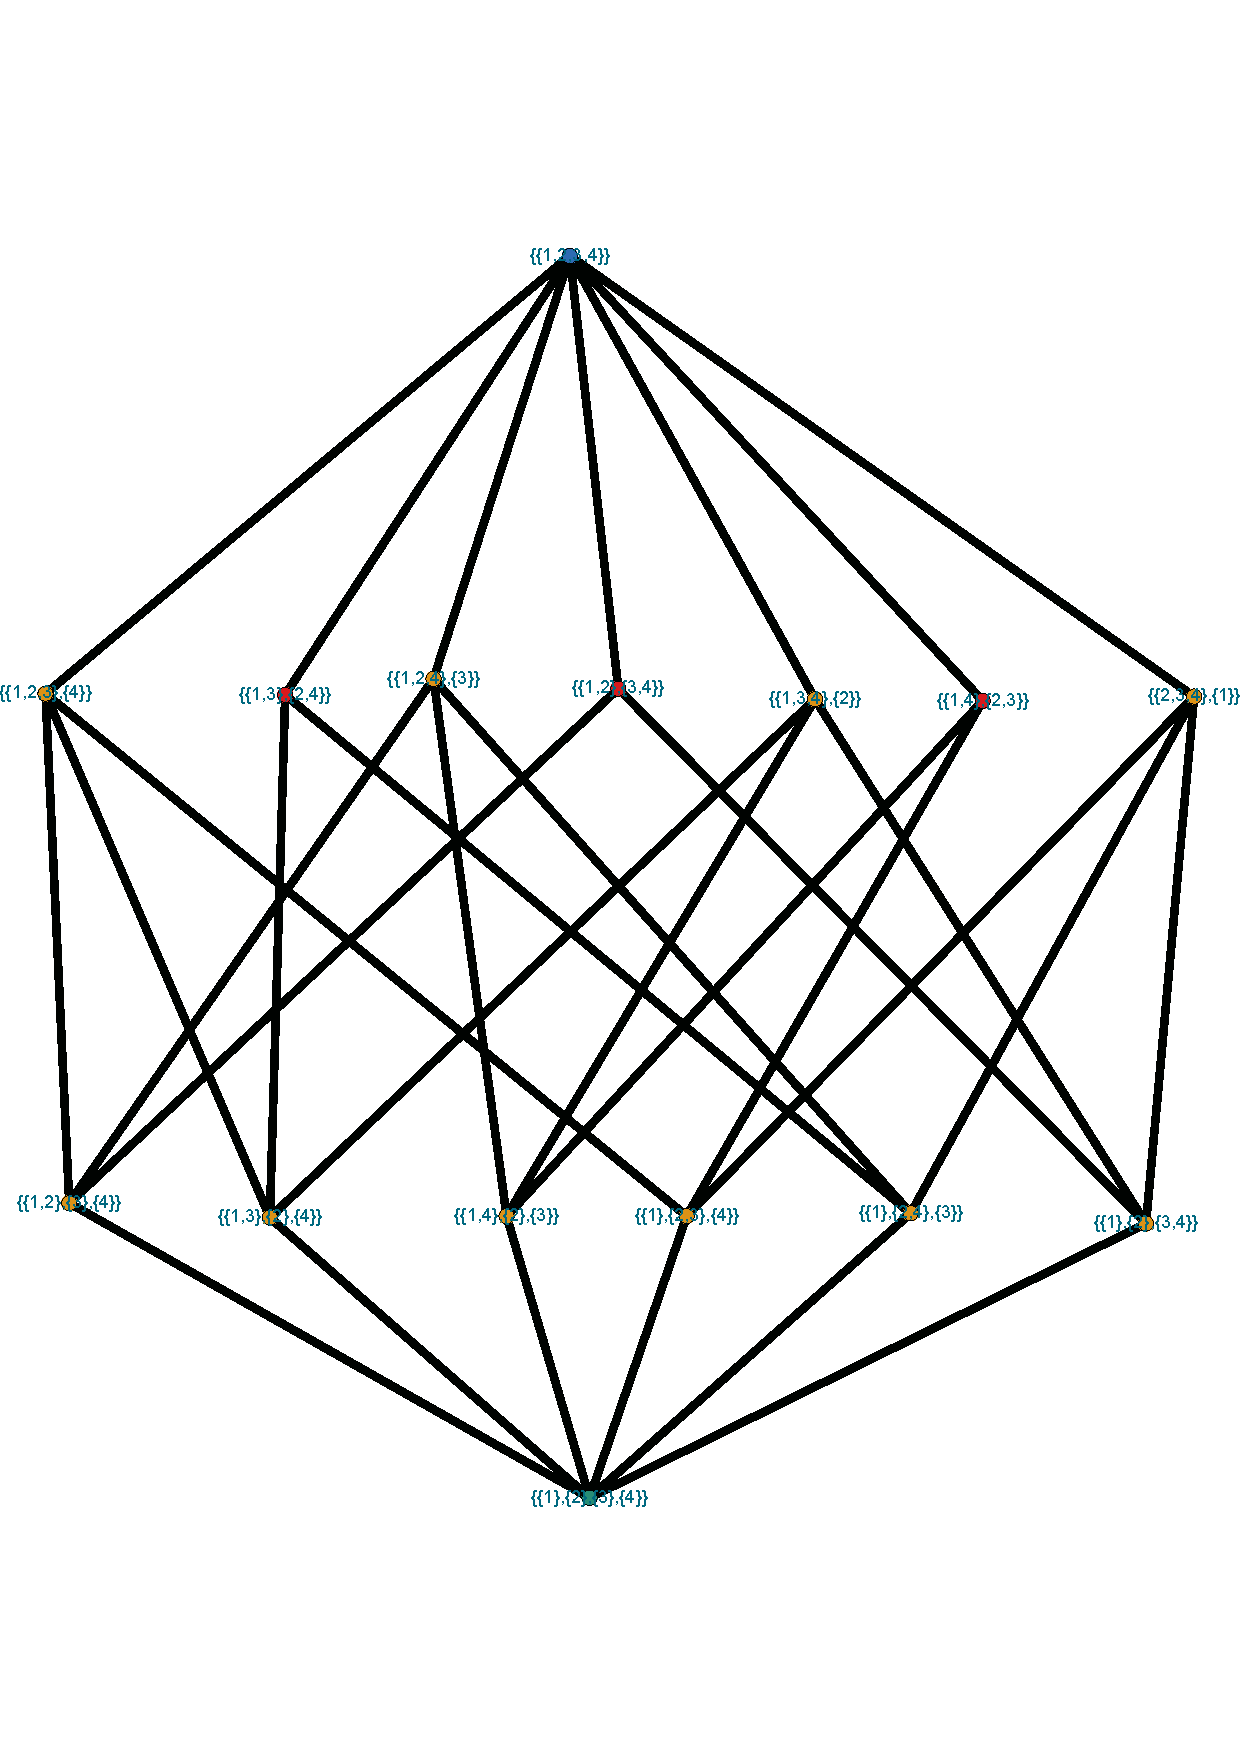
\includegraphics[height=300px,width=0.8\textwidth]{Fig-8_1.pdf}
		\caption{Hasse diagram of the partial ordering}\label{fig-8.1}
	\end{figure}
\begin{enumerate}
	\item See Figure \ref{fig-8.1}, where relation $R$ is depicted as partition explicitly.
\item As is seen in the figure, the height of the Hasse diagram is 4, and so is the size of the largest chain.
\item As is seen in the figure, the width of the Hasse diagram is 7, and so is the size of the largest antichain.
\end{enumerate}


\subsection{Chains and Antichains}

Define the partially ordered set $(\nn, \leq)$ as follows:
$x \leq y$ if $x_i \leq y_i$ for all $1 \leq i \leq n$. For example,
$(2,5,4) \leq (2,6,6)$ but $(2,5,4) \not \leq (3,1,1)$.

\begin{exercise}
  Consider the infinite partially ordered set $(\nn, \leq)$.
  \begin{enumerate}
  \item
    Which elements are minimal? Which are maximal?
  \item Is there a minimum? A maximum?
  \item Does it have an infinite chain?
  \item Does it have arbitrarily large antichains? That is, can you find an 
  antichain $A$ of size $|A| = k$ for every $k \in \N$?
\end{enumerate}
\end{exercise}
\textbf{Solution}
\begin{enumerate}
	\item \textbf{Claim.} Element $x$ such that for all $1\leq i\leq n$, $x_i=0$ is the only minimal element, and there is no maximal element.
	
	\textbf{Proof.} First suppose that there exists some element $y$, $\exists i ,1\leq i\leq n$ such that $y_i>0$. Then we can find an element $y'=(y_1,y_2,\cdots,y_i-1,\cdots,y_n)\leq y$, which contradicts with the fact that $y$ is minimal.
	
	Then suppose that there exists some maximal element $z=(z_1,z_2,\cdots,z_i,\cdots,z_n)$. Then we can find an element $z'=(z_1,z_2,\cdots,z_i+1,\cdots,z_n)\geq z$, which contradicts with the fact that $z$ is maximal. \qed
	
	Therefore the only minimal element is $(0,0,\cdots,0)$ and there is no maximal element.
	\item \textbf{Claim.} $x_0=(0,0,\cdots,0)$ is a minimum element, and there is no maximum element.
	
	\textbf{Proof.} For any $x\in\nn $, $\forall i$ in $1\leq i\leq n$, $0\leq x_i$. That is, $\forall x\in\nn$, $x_0\leq x$. Thus $x_0$ is the minimum element.
	
	Since there is no maximal element, there is no maximum element is eay to see.\qed
	\item Yes it does have an infinite chain. Or it is better to say it has infinitely many infinite chains. For example, $\{(0,0,\cdots,0),(1,0,\cdots,0),(2,0,\cdots,0),\cdots\}$ is one infinite chain. And if we remove finite elements from this chain, still we get an infinite chain. We have infinite ways to remove finite elements, so there are infinitely many infinite chains.
	\item Yes it does when $n\geq2$. But according to the definition of antichain, the smallest size of an antichain is 2 since two elements have to be distinct to be incomparable. So it is better to say that we can find an 
	antichain $A$ of size $|A| = k$ for every $k \in \N\setminus\{1\}$.
	
	\textbf{Proof.} When $n=1$, every element in $\nn$ is comparable, there is no antichain.
	
	When $n\geq2$, we can always find such an antichain of size $k$: $\{(k-1,0,0,\cdots,0),(k-2,1,0,\cdots,0),\cdots,(0,k-1,0,\cdots,0)\}$ for every $k \in \N\setminus\{1\}$.\qed
\end{enumerate}

\begin{exerciseD} 
  Does every infinite subset $S \subseteq \nn$ contain
  an infinite chain?
\end{exerciseD}

\textbf{Solution.} There are $n$ dimensions in each element. We denote the element as:
$$x=(v_1, v_2, \cdots, v_n)$$
Consider a subset of $S$ in which the $i^{th}$ dimension value of its element is a given constant:
 $$S_{v_i=c} = \{x\big|x\in S,v_i=c\}$$
 Consider the elements number of this subset. If $|S_{v_i=c}|$ is infinite, then we only have to prove $S_{v_i=c}\subseteq \nn$ contain an infinite chain. Therefore, without loss of generalization, we assume for every $i$ and $c$, $|S_{v_i=c}|$ is not infinite:
 $$|S_{v_i=c}|<\infty \quad ,i\in \{1,2,\cdots,n\}, c\in \mathbb{N}$$
 Because $S$ is an infinite set, then, for any sufficiently large $k$:

 $$\begin{aligned}
 |S_{v_i\leq k}|&=\big|\{x|x\in S, v_i\leq k\}\big| < \infty\\
 |S_{v_i> k}|&=|S|-|S_{v_i\leq k}| = \infty
 \end{aligned}$$
 Suppose we find a chain of finite size in $S_{v_i\leq k}$, and the maximal element in this chain is $(m_1,m_2,\cdots,m_i,\cdots,m_n)$, $m_i\leq k$. According to our assumption, for each $j\neq i$:
 $$|S_{v_i\geq k, v_j< m_j}|=\big|\{x|x\in S, v_i\geq k, v_j< m_j\}\big|<\infty$$ 
 Therefore, there are infinite elements larger than the maximal element in the chain:
 $$\big|\{x|x\in S, v_i\geq k, v_j\geq m_j \text{ for each $j\neq i$}\}\big|=\infty$$
 We randomly choose one element $(m'_1,m'_2,\cdots,m'_i,\cdots,m'_n)$ and add it to the chain. Then we update the value of $k$, let $k:=m'_i$. In this way we can continue this procedure indefinitely and find an infinite chain.
%--------------------------- END ---------------------------

\begin{exercise}
  Show that $(\nn,\leq)$ has no infinite antichain. \textbf{Hint.} Use 
  the previous exercise.
\end{exercise}
\textbf{Proof.} Suppose that $(\nn,\leq)$ has an infinite antichain. Then the infinite antichain itself is an infinite subset of $\nn$, and this infinite subset does not contain an infinite chain. This contradicts with the conclusion of \textbf{Exercise 8.3}.\qed



Consider the induced ordering on $\{0,1\}^n$. That is, for $x,y\in \{0,1\}^n$
we have $x \leq y$ if $x_i \leq y_i$ for every coordinate $i \in [n]$.

\begin{exercise}
 Draw the Hasse diagrams of $(\{0,1\}^n, \leq)$ for $n=2,3$.
\end{exercise}
\begin{proof}
  The figures are as follows.
\begin{figure}[htbp]
    \centering
    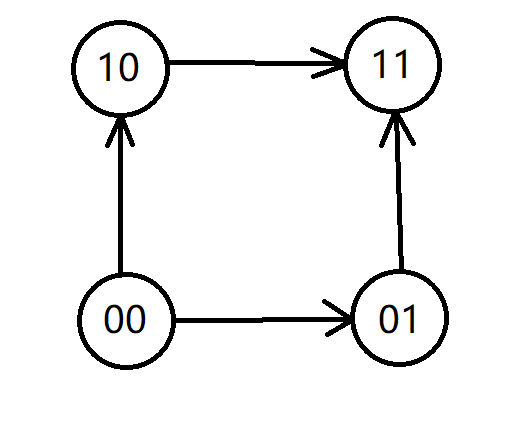
\includegraphics[width=0.4\textwidth]{2.png}
    \caption{The Hasse diagram of $(\{0,1\}^n, \leq)$ for $n=2$}
\end{figure}
\begin{figure}[htbp]
    \centering
    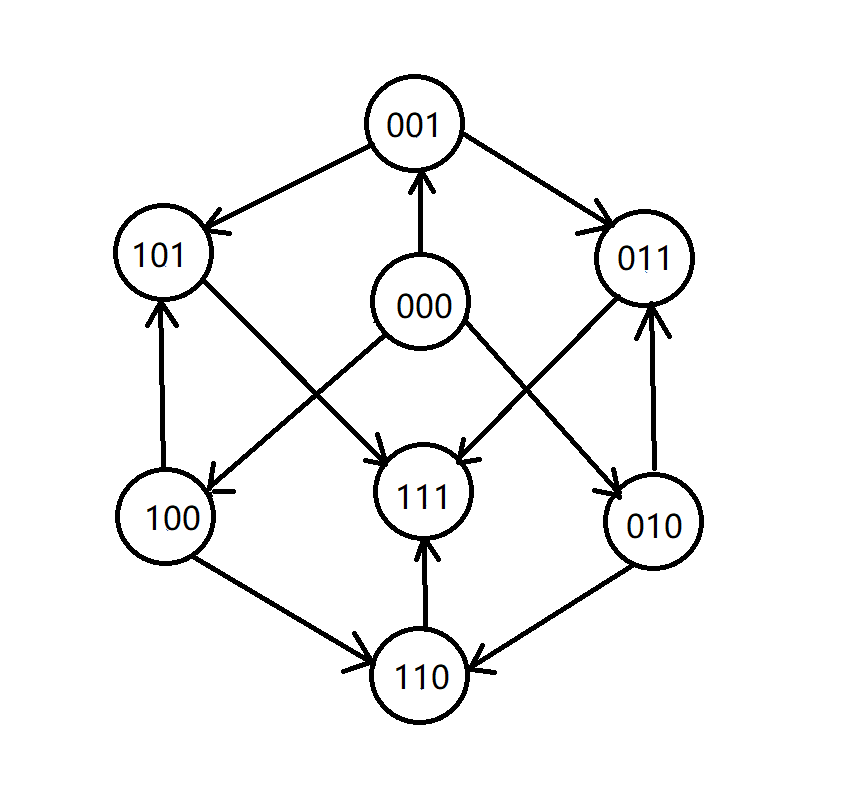
\includegraphics[width=0.4\textwidth]{3.png}
    \caption{The Hasse diagram of $(\{0,1\}^n, \leq)$ for $n=3$}
\end{figure}
\end{proof}
\begin{exercise}
  Determine the maximum, minimum, maximal, and minimal elements of
  $\{0,1\}^n$.
\end{exercise}
\begin{proof}
  maximum$:111\cdots 1$\par
  minimum$:000\cdots 0$\par
  maximal$:111\cdots 1$\par
  minimal$:000\cdots 0$\par
\end{proof}

\begin{exercise}
  What is the longest chain of $\{0,1\}^n$?
\end{exercise}
\begin{proof}
  The length of the longest chain is $n+1$. \par
  There are $n!$ longest chains. Here is an example: $000\cdots 0 \rightarrow 000 \cdots 01 \rightarrow 000 \cdots 011 \rightarrow \cdots \rightarrow 011 \cdots 11 \rightarrow 111 \cdots 11$.
\end{proof}
\begin{exerciseDD}
  What is the largest antichain of $\{0,1\}^n$?
\end{exerciseDD}

\textbf{Solution.}
\begin{figure}[htbp]
    \centering
    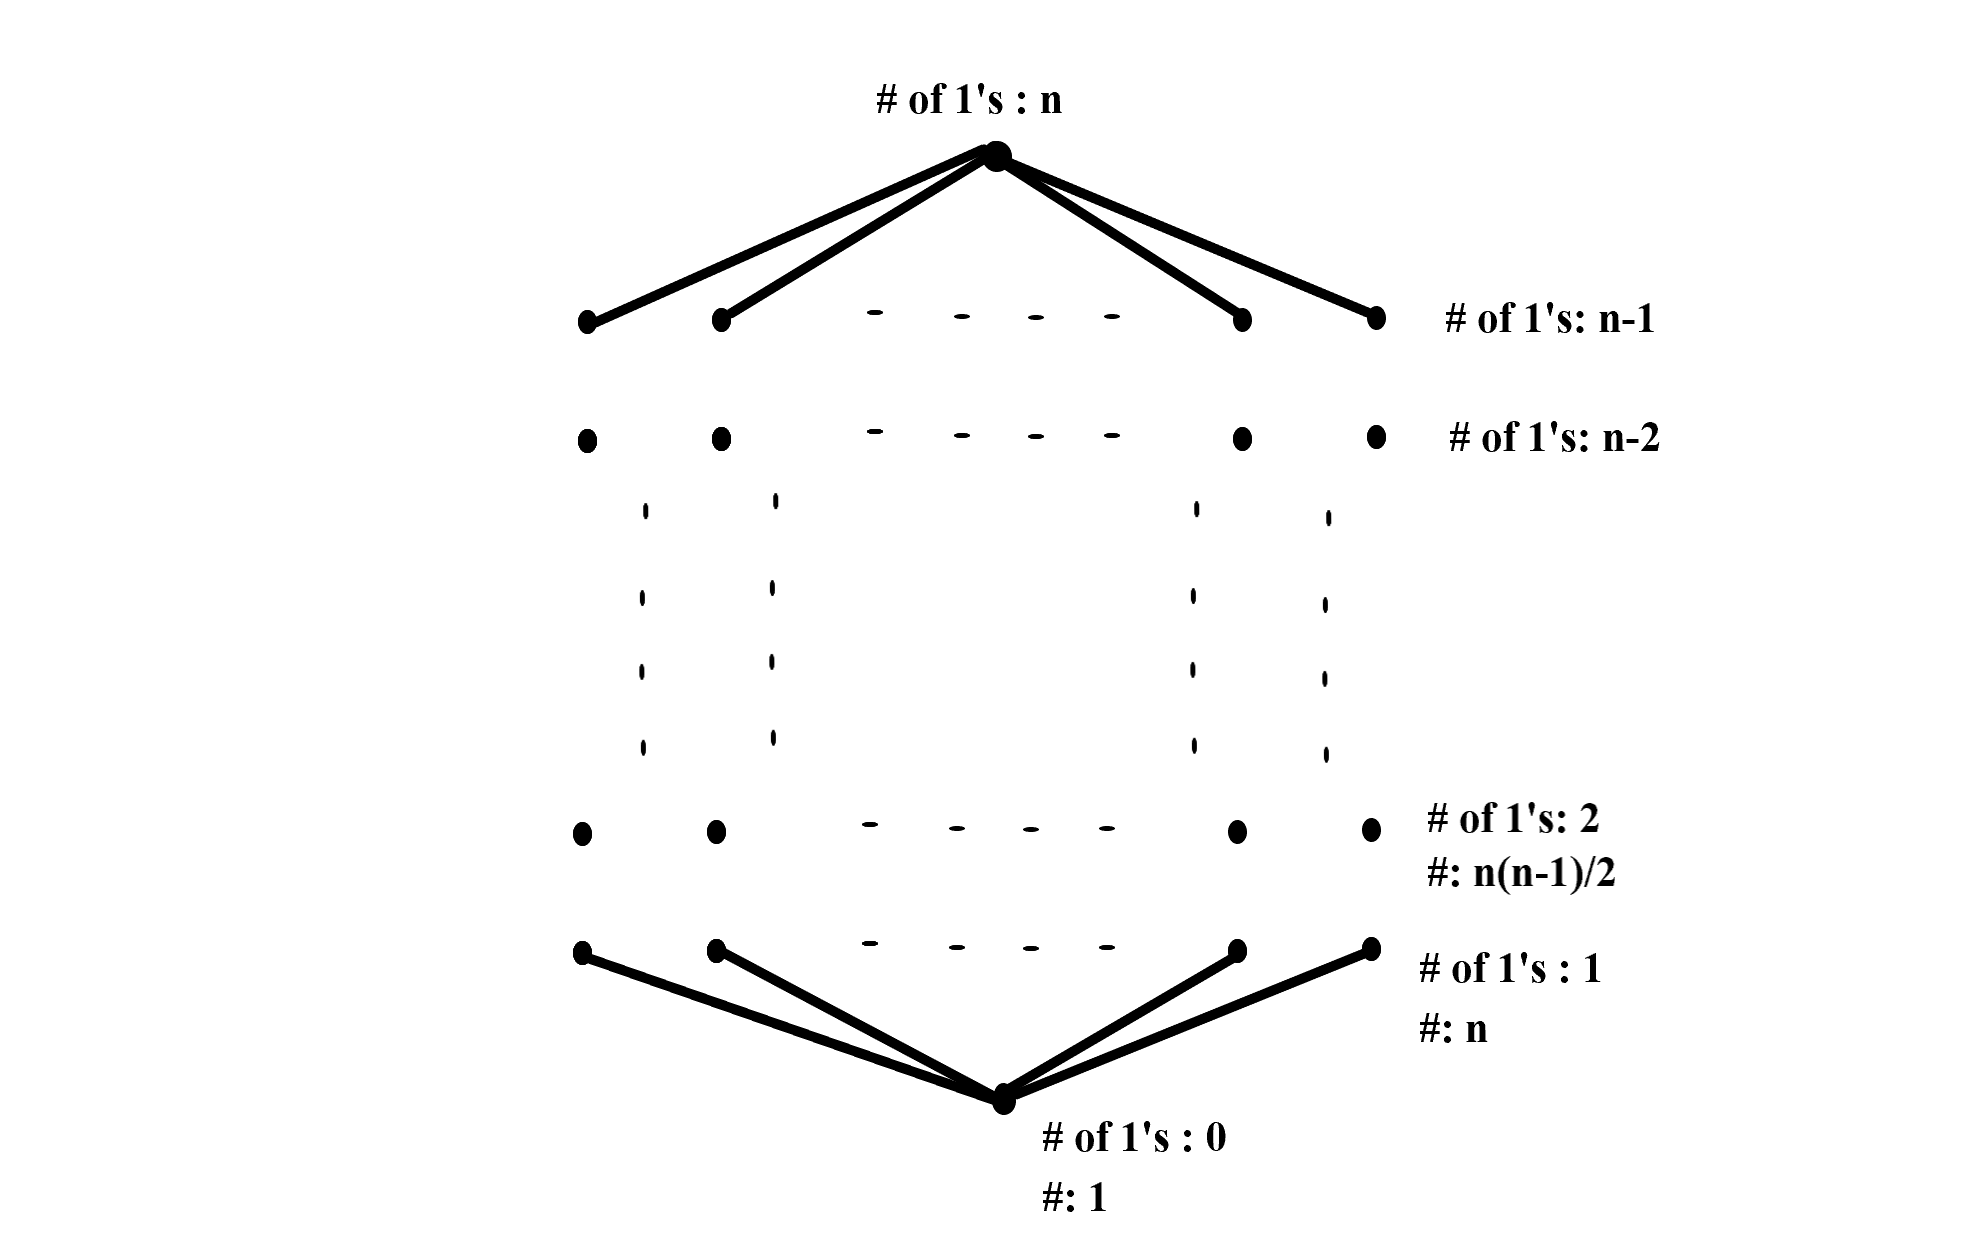
\includegraphics[width=1\textwidth]{p4.png}
    \caption{The Hasse diagram of $(\{0,1\}^n, \leq)$}
\end{figure}
	As shown in the picture, the Hasse diagram of $\{0,1\}^n$ can be divided into $n + 1$ layers. Since the number of $1$'s in each layer increases from $0$ to $n$, we have the number of nodes of each layer equal to $\binom{n}{k}$, with $0 \leq k \leq n$. Thus, the largest antichain should be $\{x|x \in \{0,1\}^n, \text{number of $1$'s in $x$ is} \lfloor \frac{n}{2} \rfloor\}$.
  \begin{proof}
    Number all the layers in the Hasse diagram $0$ to $n$ from bottom to top. By mathematical induction, we can easily derive that the the number of $1$'s in the node of $i^{th}$ layer is $i$.
  \end{proof}


\end{document}
